\documentclass{article}
\usepackage{graphicx} % Required for inserting images
\usepackage{amsmath}
\usepackage{comment}

\title{G3DCV}
\author{RICCARDO ZULIANI}
\date{August 2023}

\begin{document}

\maketitle

\section{Background Foreground Segmentation Part}
\begin{itemize}
    \item \textbf{Gain and Bias:} gain control contrast and bias control brightness
    \item \textbf{Log Transformation:} useful to compress the dynamic range for images with large variation in pixel values
    \item \textbf{Gamma Transformation:} same as lag but more flexible due to its parameter
    \item \textbf{Contrast Enchancement:} simpliest picewise-linear transformation (sigmoid shape)
    \item \textbf{Thresholding:} \(t\) is a constant defined for the whole image, if it depends on spartial coordinates, the process is referedd as adaptive thresholding
    \item \textbf{Image Histogram:} allow us to analyse problems in the intensity distribution of an image. Is the empirical distribution of image intensities.
    \item \textbf{Histogram Equalization:} maximize the intensity range of the image to catch both dark and bright details. Mapping function to obtain a uniform distribution. approximation of PDF
    \item \textbf{Histogram for Thresholding:} a common problem is to automatically find good threshold \(t\) that separates well dark from well bright areas. Thresholding is essentially a clustering problem in which two clusters are sought. The idea is to find optimum threshold so that the variance of each class (\textit{within-class-variance}) is minimized. Nobuyuki Otsu demonstrated that the optimal \(T\) that minimizes the \textit{within-class-variance} also maximize the \textit{between-class-variance}

    \par\noindent\rule{\textwidth}{0.5pt}
    \par

    \item \textbf{Linear filter:} consist of a neighbourhood and a predefined operation that is performed on the image pixels. It can be described in terms of correlation and convolution
    \item \textbf{Correlation:} moving a filter mask over a signal and computing the sum of products at each location
    \item \textbf{Convolution}: like correlation but the filter mask is roteated by 180 degrees.
    \item \textbf{Noise Reduction:}
    \begin{itemize}
        \item Gaussian-filter
        \item Median-filter: median intensity value of that pixe for its neighborhood
        \item Max-filter: brightest intensity value in the neighbourhood
        \item Min-filter: darkest intensity value in the neighbourhood
    \end{itemize}
    \item \textbf{Sharpening filters:} highlight transitions in intensity
    \begin{itemize}
        \item Unsharp masking
        \item First order derivative: thick edges because the derivative is non zero along a ramp
        \item Second order derivative (better): double edge one pixel tick, separated by zeros
    \end{itemize}
    \item \textbf{Laplacian Operators:} highlights intensity discontinuities in image and deemphasizes regions with slowly varying intensity levels


    \par\noindent\rule{\textwidth}{0.5pt}
    \par




    \item \textbf{Color characteristics}
    \begin{itemize}
        \item \textit{Brightness:} how strong is the light regardless the color
        \item \textit{Hue:} dominant wavelength in a mixture of light waves
        \item \textit{Saturation:} the relative purity of the amount of white light mixed with a hue
    \end{itemize}
    \item \textbf{Additive mixing:} from RGB color added together we obtain secondary color
    \item \textbf{Subtractive synthesis:} primary color is defined as one that subtracts or absorbs a primary color
    \item \textbf{RGB:} 3D space, additive mixing, can't represent all colors
    \item \textbf{CMY (Cyan, Magenta, Yellow) and CMYK (Cyan, Magenta, Yellow, Black)} 3D space, subtractive mixing, can't represent all colors
    \item \textbf{HSI (Hue, Saturation, Intensity):} hue is an angle
    \item \textbf{YUV:} similar to HSI but the color vector is parametrized by \(u,v\)
    \item \textbf{Smoothing and Sharpening} convolutions can also be applied to color images for smoothing and/or sharpening
    \item \textbf{LAB color code}: LAB color space expresses color variations across three channels. One channel for brightness and two channels for color:
    \begin{itemize}
        \item L-channel: representing lightness in the image
        \item a-channel: representing change in color between red and green
        \item b-channel: representing change in color between yellow and blue
    \end{itemize}
    \item \textbf{Adaptive histogram equalization:}  is a computer image processing technique used to improve contrast in images. It differs from ordinary histogram equalization in the respect that the adaptive method computes several histograms, each corresponding to a distinct section of the image, and uses them to redistribute the lightness values of the image. It is therefore suitable for improving the local contrast and enhancing the definitions of edges in each region of an image.
    However, AHE has a tendency to overamplify noise in relatively homogeneous regions of an image. A variant of adaptive histogram equalization called contrast limited adaptive histogram equalization (CLAHE) prevents this by limiting the amplification. 
    \item \textbf{CLAHE (Contrast Limited Adaptive Histogram Equalization):} Ordinary AHE tends to overamplify the contrast in near-constant regions of the image, since the histogram in such regions is highly concentrated. As a result, AHE may cause noise to be amplified in near-constant regions. Contrast Limited AHE (CLAHE) is a variant of adaptive histogram equalization in which the contrast amplification is limited, so as to reduce this problem of noise amplification. In CLAHE, the contrast amplification in the vicinity of a given pixel value is given by the slope of the transformation function. This is proportional to the slope of the neighbourhood cumulative distribution function (CDF) and therefore to the value of the histogram at that pixel value. CLAHE limits the amplification by clipping the histogram at a predefined value before computing the CDF. This limits the slope of the CDF and therefore of the transformation function. The value at which the histogram is clipped, the so-called clip limit, depends on the normalization of the histogram and thereby on the size of the neighbourhood region. Common values limit the resulting amplification to between 3 and 4. 
    \item \textbf{HSV} (hue, saturation, value) colorspace is a model to represent the colorspace similar to the RGB color model. Since the hue channel models the color type, it is very useful in image processing tasks that need to segment objects based on its color. Variation of the saturation goes from unsaturated to represent shades of gray and fully saturated (no white component). Value channel describes the brightness or the intensity of the color.
    
    \par\noindent\rule{\textwidth}{0.5pt}
    \par
    
    \item \textbf{Preliminaries:} considering thresholded images containing only black and white pixels
    \item \textbf{Set translation:} creates a new set by translating every point of the initial set by the same amount \(z(z_1,z_2)\)
    \item \textbf{Set reflection} creates a new set whose coordinates are replaced with \((-x, -y)\)
    \item \textbf{Structuring elements:} small set of sub-images used to probe an image under study for properties of interest
    \item \textbf{Erosion:} it erodes away the boundaries of foreground object. A pixel in the original image (either 1 or 0) will be considered 1 only if all the pixels under the kernel is 1, otherwise it is eroded (made to zero). All the pixels near boundary will be discarded depending upon the size of kernel. So the thickness or size of the foreground object decreases or simply white region decreases in the image. It is useful for removing small white noises (as we have seen in colorspace chapter), detach two connected objects etc.
    \item \textbf{Dilatation:} It is just opposite of erosion. Here, a pixel element is '1' if at least one pixel under the kernel is '1'. So it increases the white region in the image or size of foreground object increases. Normally, in cases like noise removal, erosion is followed by dilation. Because, erosion removes white noises, but it also shrinks our object. So we dilate it. Since noise is gone, they won't come back, but our object area increases. It is also useful in joining broken parts of an object.
    \item \textbf{Idea:} by combining operations, somehow the effect cancel out noise in region where I'm not interested to change the shape of the object, out some pixel will change
    \item \textbf{Opening (erosion followed by a dilatation):} smoothens the contour of an object, eliminates thin protrusions
    \item \textbf{Closing (dilatation followed by a erosion):} smoothens sections of contours, fuses narrow breaks and long thin gulfs, eliminates small holes, fills gaps in the contour
    \item \textbf{Grayscale morphology:} erosion, dilatation, opening and closing can also be defined for grayscale images
    \item \textbf{Erosion:} computes the minimum intensity values over every neighborhood of (x,y), the resulting image is darker and the size of bright features is in general reduced
    \item \textbf{Dilatation:} gives opposite result wrt erosion, The resulting image is brighter, bright features are thickened and the intensities of the dark features is reduced
    \item \textbf{Opening:} \textit{attenuate bright features} and has negligible effect on the dark features and the background of the image
    \item \textbf{Closing:} \textit{attenuate dark features} and as negligible effect on the bright features and the background of the image
    \item \textbf{Morphological Gradient:} is the difference between dilation and erosion of an image
    \item \textbf{Top-hat:} is the difference between input image and Opening of the image
    \item \textbf{Bottom-hat or Black-hat:} is the difference between the closing of the input image and input image
\end{itemize}

\newpage
\section{Marker Detector Part}
\begin{itemize}
    \item \textbf{Features:} location of sudden change in intensity. Useful since information content is high, invariant to change of viewpoint or illumination, reduces computational burden
    \item \textbf{Good Feature} is invariant to:
    \begin{itemize}
        \item Viewpoint
        \item Lighting conditions
        \item Object deformations
        \item Partial occlusions
    \end{itemize}
    And should be unique and easy to be found and extracted
    \item \textbf{Edges:} edges are pixels at which the intensity of an image function changes abruptly
    \item \textbf{Edge detection:} find image pixels that present abrupt changes in intensity
    \item \textbf{Edge models:}
    \begin{itemize}
        \item \textit{Step edge:} from 0 to 1 in a single pixel
        \item \textit{Ramp edge:} blurring while changing intensity
        \item \textit{Roof edge:} rise and goes down within a bit pixels 
    \end{itemize}
    \item \textbf{Derivatives:}
    \begin{itemize}
        \item The magnitude of the first derivative can be used to detect the presence of an edge at a point in an image
        \item \textit{Gradient} finds the strength and direction at point\((x,y)\)
        \item \textit{Magnitude} is the amount of change in that direction
        \item \textit{Computing the gradient:} approximation of the partial derivatives over a neighborhood about a point is required. 
        \item \textit{Prewitt operators}
        \item \textit{Sobel operators} is a slight variation of Prewitt since it uses a weight of 2 in the center coefficient, better noise-suppression 
    \end{itemize}
    \item \textbf{Marr-Hildrreth Edge Detection} Laplacian of Gaussian instead of Sobel mask\
    \begin{itemize}
        \item \textit{The Gaussian} blur the image reducing the intensity of structures thus reducing the artefacts
        \item \textit{The Laplacian} responds equally in intensity in any direction
        \item \textit{Zero-Crossing} a zero crossing in a 3x3 neighbourhood centered at \(p\) implies that the signs of at least two of uts opposing neighbouring pixels must differ
    \end{itemize}
    \item \textbf{Marr-Hildrreth Edge Detection Algorithm}
    \begin{itemize}
        \item Blur the image with Gaussian filter
        \item Compute the Laplacina of the blurred image
        \item Find the zero crossing: very sensible to noise, in addition to the previous requirements of zero crossing we require also the absolute value of their numerical; difference must exceed a threshold T
    \end{itemize}

    \item \textbf{Canny Edge Detector}
    \begin{itemize}
        \item Smooth the input image with a 2D Gaussian filter
        \item Compute the gradient magnitude and angle of the smoothed image reduce the noise
        \item Non-maxima suppression to the gradient magnitude: for each pixel check the neighbours along the direction of the gradient, if the intensity of the gradient is less than at least one of the two neigh, it must be suppressed
        \item Use double thresholding and connectivity analysis to detect and link edges (Hysteresis thresholding): This stage decides which are all edges are really edges and which are not. For this, we need two threshold values, minVal and maxVal. Any edges with intensity gradient more than maxVal are sure to be edges and those below minVal are sure to be non-edges, so discarded. Those who lie between these two thresholds are classified edges or non-edges based on their connectivity. If they are connected to "sure-edge" pixels, they are considered to be part of edges. Otherwise, they are also discarded.
    \end{itemize}


    \par\noindent\rule{\textwidth}{0.5pt}
    \par

    \item \textbf{Harris Corner Detector} see on the slides
    \item \textbf{SIFT} see on the slides


    \par\noindent\rule{\textwidth}{0.5pt}
    \par


    
    \item \textbf{cv.findContours(mask\_thresh, cv.RETR\_TREE, \\cv.CHAIN\_APPROX\_SIMPLE)}:
    \begin{itemize}
        \item \textit{cv.RETR\_TREE:} retrieves all of the contours and reconstructs a full hierarchy of nested contours
        \item \textit{cv.CHAIN\_APPROX\_SIMPLE:} compresses horizontal, vertical, and diagonal segments and leaves only their end points. For example, an up-right rectangular contour is encoded with 4 points
    \end{itemize}
    Contours can be explained simply as a curve joining all the continuous points (along the boundary), having same color or intensity. The contours are a useful tool for shape analysis and object detection and recognition.

    Algorithm, "Marching Squares" algorithm, adapted for digital image processing:
    \begin{itemize}
        \item \textit{Image Traversal:} The algorithm starts by traversing the binary image pixel by pixel. It looks for edge points, where an edge is defined as a transition from background (black) to object (white) or vice versa.
        \item \textit{Starting Point:} When an edge point is found, it becomes the starting point of a contour. The algorithm follows the neighboring pixels in a clockwise manner until it reaches the starting point again, forming a closed contour.
        \item \textit{Tracing Contour:} As the algorithm follows the contour, it tracks the visited pixels' locations. It also marks these visited pixels in a separate "visited" map to ensure that each pixel is only considered once.
        \item \textit{Pixel Connectivity:} The algorithm's direction of traversal is determined by the pixel connectivity. It can be either 4-connectivity or 8-connectivity, where 4-connectivity considers only the horizontal and vertical neighbors, and 8-connectivity considers all eight neighboring pixels.
        \item \textit{Stopping Conditions:} The traversal continues until the algorithm returns to the starting point, completing the contour. If multiple contours are present in the image, the algorithm repeats the traversal process from other unvisited edge points until all contours are found.
        \item \textit{Hierarchy:} If requested, the algorithm can also compute and return information about the hierarchy of contours. This is useful for detecting nested contours and understanding how contours are connected.
        \item \textit{Output:} The algorithm outputs a list of contours, where each contour is represented as a sequence of points. The contour points are typically sampled with a certain level of accuracy, preserving the contour's essential shape.
    \end{itemize}

    \item \textbf{cv.contourArea():} The function computes a contour area. Similarly to moments , the area is computed using the Green formula. Green's Theorem is a fundamental result in vector calculus that establishes a relationship between line integrals around a closed curve and double integrals over the region enclosed by that curve

    \item \textbf{cv.approxPolyDP(cnt, 0.015 * cv.arcLength(cnt, closed=True), closed=True)}:
    \begin{itemize}
        \item Approximates a curve or a polygon with another curve/polygon with less vertices so that the distance between them is less or equal to the specified precision.
        \item Douglas-Peucker algorithm is an algorithm that decimates a curve composed of line segments to a similar curve with fewer points
        \begin{itemize}
            \item The starting curve is an ordered set of points or lines and the distance dimension \(\epsilon > 0\).
            \item The algorithm recursively divides the line. Initially it is given all the points between the first and last point. It automatically marks the first and last point to be kept. It then finds the point that is farthest from the line segment with the first and last points as end points; this point is obviously farthest on the curve from the approximating line segment between the end points. If the point is closer than \(\epsilon\) to the line segment, then any points not currently marked to be kept can be discarded without the simplified curve being worse than \(\epsilon\).
            \item If the point farthest from the line segment is greater than \(\epsilon\) from the approximation then that point must be kept. The algorithm recursively calls itself with the first point and the farthest point and then with the farthest point and the last point, which includes the farthest point being marked as kept. 
            \item When the recursion is completed a new output curve can be generated consisting of all and only those points that have been marked as kept.
        \end{itemize}
    \end{itemize}

    \item \textbf{cv.arcLength(cnt, closed=True)}: Calculates a contour perimeter or a curve length. This step is very important, since it is the epsilon for the cv.approxPolyDP. The correct approximation of the contour depends on selection of epsilon.

    \item \textbf{cv.cornerSubPix(imgray, np.float32(approx\_cnt), winSize\_sub, zeroZone\_sub, criteria\_sub):} refines the corner locations.
    \begin{itemize}
        \item image
        \item corners
        \item winSize: 	Half of the side length of the search window. For example, if winSize=Size(5,5) , then a \((5*2+1) \times (5*2+1)=11 \times 11\) search window is used. 
        \item zeroZone: Half of the size of the dead region in the middle of the search zone over which the summation in the formula below is not done. It is used sometimes to avoid possible singularities of the autocorrelation matrix. The value of (-1,-1) indicates that there is no such a size. 
        \item criteria: Criteria for termination of the iterative process of corner refinement. That is, the process of corner position refinement stops either after criteria.maxCount iterations or when the corner position moves by less than criteria.epsilon on some iteration. 
    \end{itemize}
    Sub-pixel accurate corner locator is based on the observation that every vector from the center q to a point p located within a neighborhood of q is orthogonal to the image gradient at p subject to image and measurement noise. 

    \item \textbf{cv.convexHull():} finds the convex hull of a 2D point set using the Sklansky's algorithm, which then was found to be incorrect
    \begin{itemize}
        \item A Convex object is one with no interior angles greater than 180 degrees. A shape that is not convex is called Non-Convex or Concave.
        \item Hull means the exterior or the shape of the object.
        \item Convex Hull of a shape or a group of points is a tight fitting convex boundary around the points or the shape.
    \end{itemize}


    \par\noindent\rule{\textwidth}{0.5pt}
    \par





    \item \textbf{Flow and Tracking:} track position and movement of an object across a video sequence
    \item \textbf{Motion Field:} would like to estimate the 2D velocities of the image points induced by the relative motion between the viewing camera and the observed objects. Projection of the 3D velocity field onto the image plane
    \item \textbf{Optical Flow:} observed 2D displacements of brightness patterns in the image \(E(x,y,t)\). \((x, y)\) set of pixels, \(t\) time
    \item \textbf{Brightness consistency equation:} the apparent brightness will remain constant during the movement
    \[\frac{\partial E}{\partial x} \frac{\partial x}{\partial t} + \frac{\partial E}{\partial y} \frac{\partial y}{\partial t} + \frac{\partial E}{\partial t} = 0\]
    Where:
    \begin{itemize}
        \item \(\frac{\partial E}{\partial x}\) and \(\frac{\partial E}{\partial y}\) horizontal and vertical gradient (spartial gradients computed via convolution Sobel)
        \item \(\frac{\partial x}{\partial t}\) and \(\frac{\partial y}{\partial t}\) optical flow: \(\vec{v} + (\frac{\partial x}{\partial t}, \frac{\partial y}{\partial t}) = (u,v)\)
        \item \(\frac{\partial E}{\partial t}\) image derivative across frames
    \end{itemize}
    \[(\Delta E)^T \vec{v} + E_t = 0\]
    \[E_xu + E_yv + E_t = 0\]
    We have 3 know coefficients \((x,y,t)\) and 2 unknowns \((u,v)\). This is like the equation of a line

    \item \textbf{The aperture problem:} the component of the optical flow orthogonal to the spartial image gradient is not constrained by the image brightness constancy equation. Thus only the flow in the gradient direction can be determined

    \item \textbf{Computing OF with Lukas Kanade flow:}
    \begin{itemize}
        \item Based on the spartial and temporal variations of the image brightness at all pixels
        \item Used to compute dense flow
        \item One equation per pixel is not enough so we make an additional assumption: the optical flow is well approximated by a constant vector within any small patch of the image plane
        \item Suppose that we use a patch \(Q\) with size \(N \times N\) (like \(5 \times 5\)), supposing that \((u,v)\) is constant for every pixel in \(Q\) we obtain a system of 25 equations in 2 unknowns, which is over-determined. A better solution is obtained with least square fit method thst is suitable for over-estimated system.

        \begin{figure}[!htb]
             \centering
             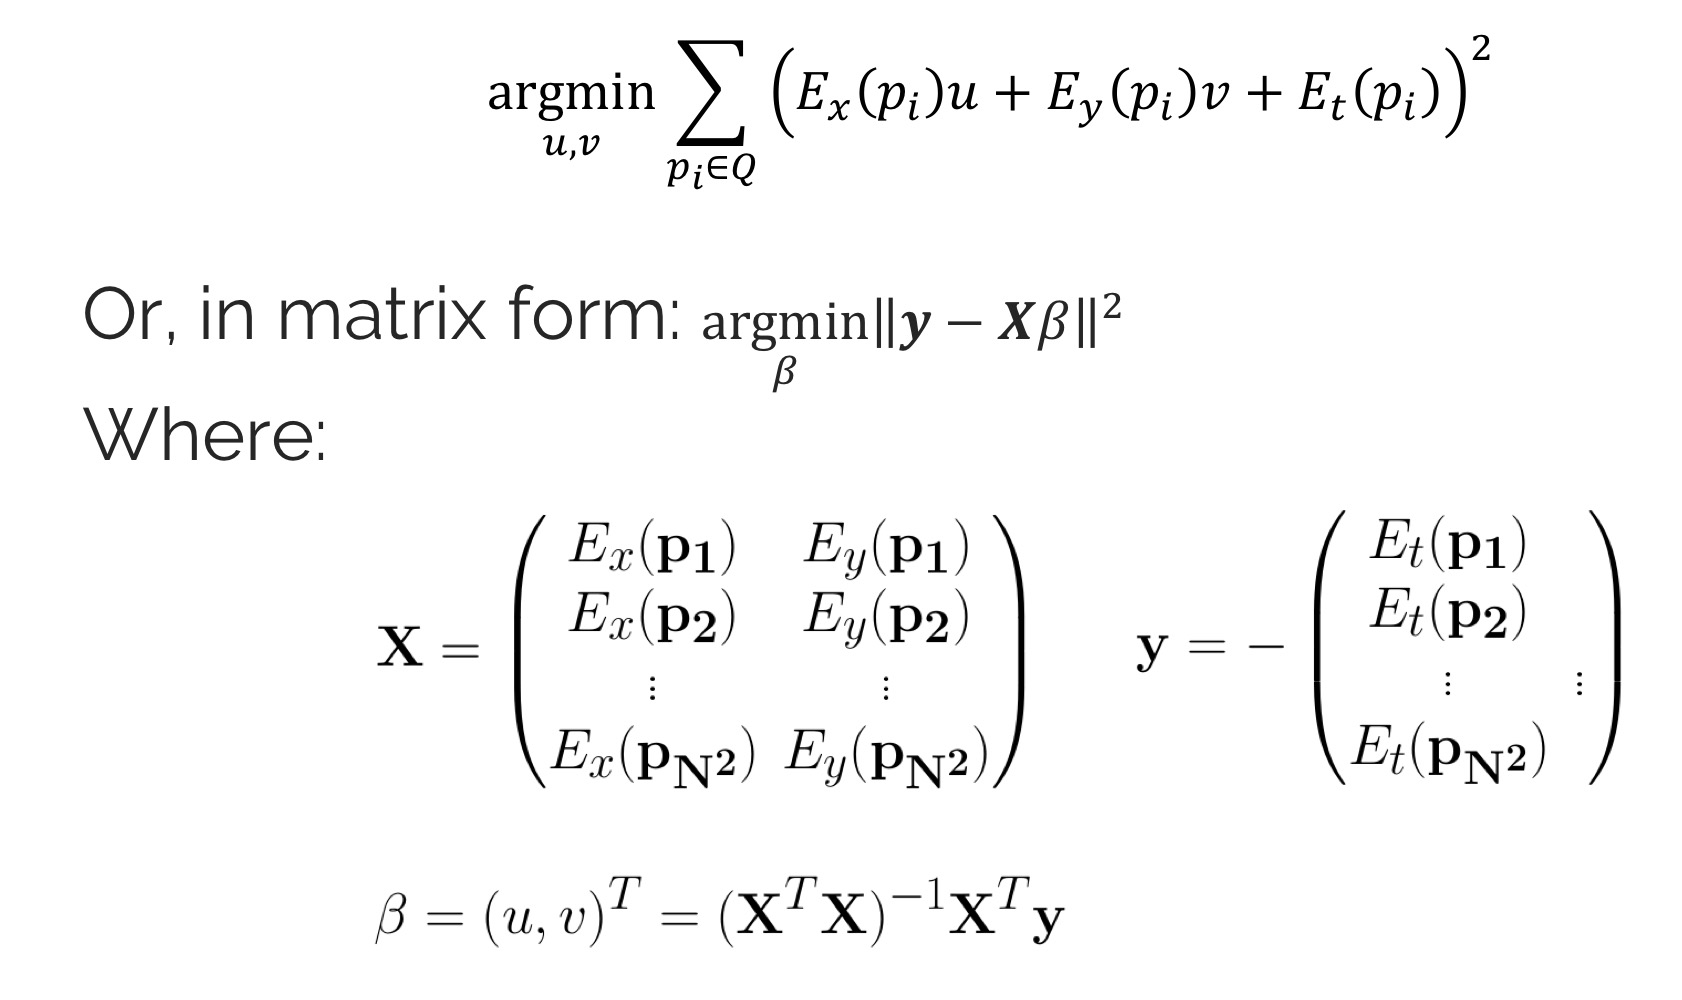
\includegraphics[width=1\linewidth]{IMG_1042.jpeg}
        \end{figure}
        \item Solving this least square problem depends by inverting the matrix \(A = X^TX\) where:
        \begin{itemize}
            \item \(A\) should be invertible, thus bot eigenvalues must be not zero
            \item \(A\) should be well conditioned, large \(\lambda_1\) and \(\frac{\lambda_1}{\lambda_2}\) not too large
        \end{itemize}
        \begin{figure}[!htb]
             \centering
             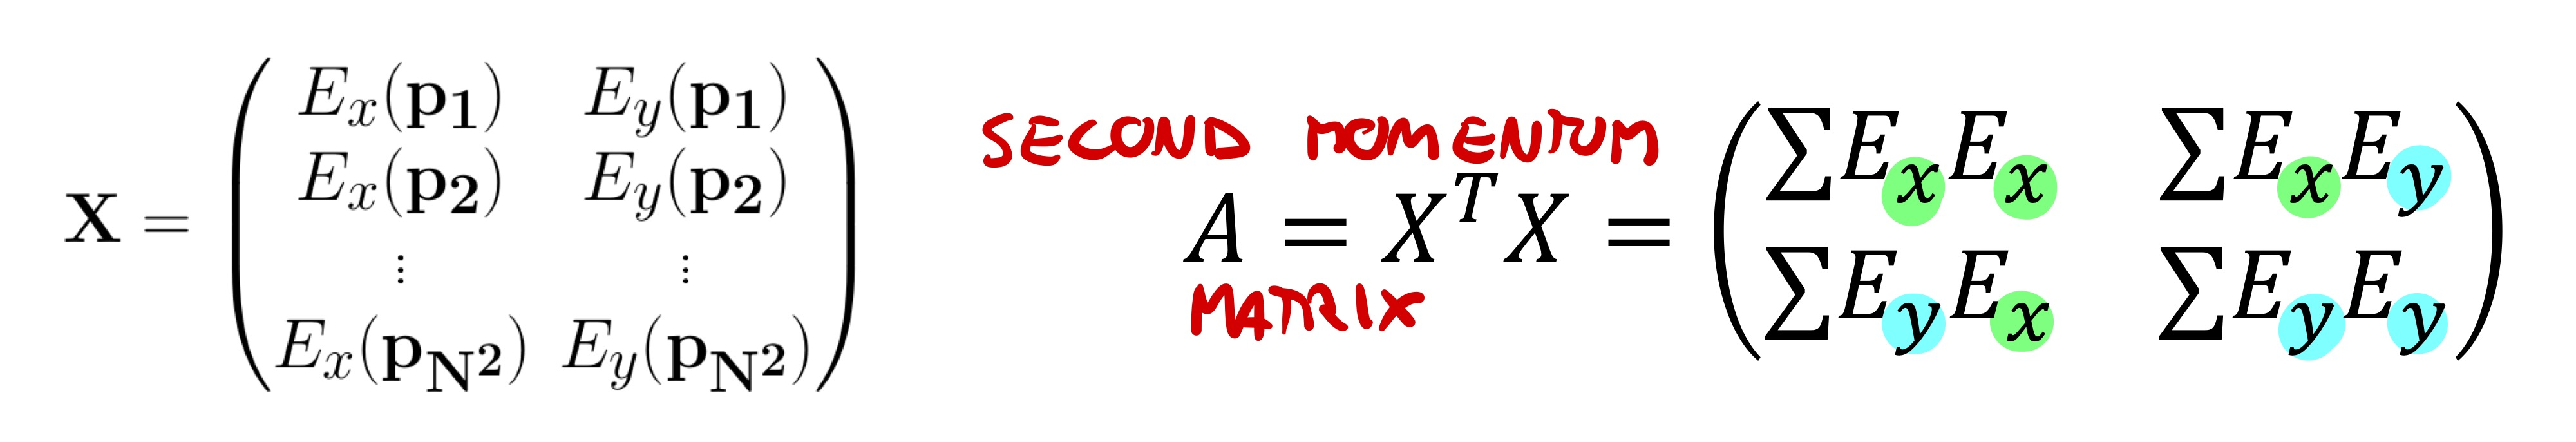
\includegraphics[width=1\linewidth]{IMG_1043.jpeg}
        \end{figure}
        \item \(A\) is exactly the structure tensor used in the Harris corner detector
        \item Corners are places in which bot \(\lambda_1, \lambda_2\) are big and this also is the case in which the LK flow works best
        \item Aperture problem disappear at corners. \textbf{Corners are a good place to compute optical flow}
        \item Until now, we were dealing with small motions, so it fails when there is a large motion. To deal with this we use pyramids. When we go up in the pyramid, small motions are removed and large motions become small motions. So by applying Lucas-Kanade there, we get optical flow along with the scale.
    \end{itemize}

    \newpage
    \section{Pose Estimation Part}
    \begin{itemize}
        \item Points
        \item 2D Projective Space
        \item Homogeneous coordinates
        \item Ideal Points
        \item 2D lines
        \item Ideal points and the line at infinity
        \item 2D Projectivities
        \begin{itemize}
            \item 2D Translation
            \item 2D Rotation
            \item 2D Rigid Motion: rotation + translation
            \item 2D Similarity: rotation + isotopic scale + translation
            \item 2D Affine Transformation: linear transformation followed by a translation
            \item 2D Projective Transformation: homography since we work with \(P^2\), is a general non singular transformation of homogeneous coordinates
            \item Projective VS Affine: main difference is \(v^T\) this vector is responsible for the non-linear effects of the projectivity and allows such transformation to model vanishing points
        \end{itemize}
        \item Projective 3-Space: homogeneous coordinates as a 4-dimensional vector
        \item Projective transformations: is a linear transformation in \(P^3\) that can be represented by any non-singular \(4 \times 4\) matrix
        \item Rigid Motion: the euclidean transformation is a projective transformation composed by a rotation R around an axis and a translation t

        \item \textbf{Pinhole camera:} how small must be the pinhole be?
        \begin{itemize}
            \item \textit{Large pinhole:} blurring
            \item \textit{Small pinhole:} gain focus but less light passes through, diffraction effect
        \end{itemize}
        \item \textbf{Solution:} uses lenses to focuses light onto the sensor
        \item \textbf{Camera and lenses:}
        \begin{itemize}
            \item All parallel rays converge to one point on a plane located at the focal length f
            \item There is a specific distance at which the objects are in focus
            \item Rays a re reflected when passing through the lens according to Snell's law
        \end{itemize}
        \item \textbf{Distortion:} imperfect lenses may cause radial distortion
        \item \textbf{Pinhole camera model}
        \[p=\begin{pmatrix}x \\ y\\ z\end{pmatrix} \quad p'= \begin{pmatrix}u\\ v \end{pmatrix} \quad u = \frac{x}{z}f \quad v = \frac{y}{z}f\]
        \item \textbf{Projection:} when we capture a scene with a pinhole camera, we are mapping a 3D points to a 2D points according the the function \(E: R^3 \rightarrow R^2\)
        \[(x,y,z) \rightarrow \Big(\frac{x}{z}f, \frac{y}{z}f\Big)\]
        This function is not linear due to the division by \(z\)
        By using homogeneous coordinates , we can express the projection with a linear mapping \(E: P^3 \rightarrow P^2\)
        \[P' = \begin{pmatrix}
            fx \\ fy \\ z
        \end{pmatrix} = \begin{pmatrix}
            f & 0 & 0 & 0\\
            0 & f & 0 & 0\\
            0 & 0 & 1 & 0\\
        \end{pmatrix} \begin{pmatrix}
            x \\ y \\ z \\ 1
        \end{pmatrix}\]
        The division by \(z\) occurs only when we transform \(P'\) back to inhomogeneous coordinates
        \item \textbf{Principal point}
        \begin{itemize}
            \item The image reference system is usually placed at the top-left corner of the image
            \item After the projection the coordinates of \(p'\) are expressed with respect to the principal point C
        \end{itemize}
        \[P' = \begin{pmatrix}
            fx + c_xz \\ fy + c_yz \\ z
        \end{pmatrix} = \begin{pmatrix}
            f & 0 & c_x & 0\\
            0 & f & c_y & 0\\
            0 & 0 & 1 & 0\\
        \end{pmatrix} \begin{pmatrix}
            x \\ y \\ z \\ 1
        \end{pmatrix}\]


        \item \textbf{Lens Distortion:} lens distortion produces a non linear displacement of points after their projection
        \item \textbf{Modeling the lens distortion:} as a polynomial function of the radial distance form the lens center
        \item \textbf{Image undistort:} once the lens distortion parameters are known, an image can be "undistorted" ad it would be taken with a perfect pinhole camera.
        Compute the inverse wrap from the ideal undistorted image to the original distorted image according to the distortion function
        For each pixel \(u,v\) in ther target image
        \begin{itemize}
            \item Move backward in the projection chain to the retinal plane
            \[\begin{pmatrix}x'\\ y'\\ 1\end{pmatrix} = K^{-1} \begin{pmatrix}u\\ v\\ 1\end{pmatrix}\]
            \item Apply the radial distortion function to obtain \((\widetilde{x}', \widetilde{y}', 1)^T\)
            \item Move forward in the projection chain to get the coordinates in the distorted image
            \[\begin{pmatrix}u'\\ v'\\ 1\end{pmatrix} = K \begin{pmatrix}\widetilde{x}'\\ \widetilde{y}'\\ 1\end{pmatrix}\]
        \end{itemize}
        \item \textbf{Camera pose:} 
        \begin{itemize}
            \item All of this is under the assumption that object points were expressed in the camera reference system
            \item When dealing with multiple cameras it is common to represent points in a common world reference system
            \item A rotation matrix \(R\) and a translation vector \(T\) express the rigid motion from a world reference system to the camera reference system
        \end{itemize}
        \item \textbf{World to Camera} to be projected a point \(p_w \in P^3\) must be first transformed into the camera coordinate system, in 4D homogeneous coordinates we got:
        \[p= \begin{pmatrix} R & T \\ 0 & 1 \end{pmatrix}p_w\]
        \item \textbf{\(R\) and \(T\)} are called the \textbf{extrinsic parameter}
        \item \textbf{Complete projection}
        \[
        p'=\begin{pmatrix}
            f & 0 & c_x\\
            0 & f & c_y\\
            0 & 0 & 1
        \end{pmatrix}\begin{pmatrix}
            R & T
        \end{pmatrix}\begin{pmatrix}
            x_w \\ y_w \\ z_w \\ 1
        \end{pmatrix}
        \]
        \[p'=K\begin{pmatrix} R & T \end{pmatrix}\begin{pmatrix}
            x_w \\ y_w \\ z_w \\ 1
        \end{pmatrix}\]
        \item \textbf{Finite projective camera}
        \begin{itemize}
            \item Pixel may not be squared
            \item The produced image is not rectangular
        \end{itemize}
        \[P = \begin{pmatrix}
            f_x & s & c_x\\
            0 & f_y & c_y\\
            0 & 0 & 1
        \end{pmatrix}\begin{pmatrix}
            R & T
        \end{pmatrix}\]
        
    \end{itemize}


    \section{Camera Calibration Part}
    see notes.

    In addition to this, we need to some other information, like the intrinsic and extrinsic parameters of the camera. Intrinsic parameters are specific to a camera. They include information like focal length \((f_x,f_y)\) and optical centers \((c_x,c_y)\). The focal length and optical centers can be used to create a camera matrix, which can be used to remove distortion due to the lenses of a specific camera. The camera matrix is unique to a specific camera, so once calculated, it can be reused on other images taken by the same camera.

    \subsection{Used Methods}
    \begin{itemize}
        \item \textbf{findChessboardCorners():} Finds the positions of internal corners of the chessboard. 
        \item \textbf{calibrateCamera()}
        \item \textbf{getOptimalNewCameraMatrix():} The function computes and returns the optimal new camera intrinsic matrix based on the free scaling parameter. By varying this parameter, you may retrieve only sensible pixels alpha=0 , keep all the original image pixels if there is valuable information in the corners alpha=1 , or get something in between. When alpha>0 , the undistorted result is likely to have some black pixels corresponding to "virtual" pixels outside of the captured distorted image.
        \item \textbf{undistort():} Transforms an image to compensate for lens distortion. The function transforms an image to compensate radial and tangential lens distortion.
        \item \textbf{solvePnP():} returns the rotation and the translation vectors that transform a 3D point expressed in the object coordinate frame to the camera coordinate frame
        \item \textbf{projectPoints():} The function computes the 2D projections of 3D points to the image plane, given intrinsic and extrinsic camera parameters. 
        \item \textbf{Alternative methods to projectPoints() is:}
        \begin{itemize}
            \item Run calibrateCamera to obtain the \(3 \times 3\) matrix as cameraMatrix, a \(4 \times 1\) matrix as distCoeffs, and rvecs and tvecs that are vectors of \(3 \times 1\) rotation(R) and \(3 \times 1\) transformation(t) matrices.
            \item Run Rodriguez with the \(3 \times 1\) rotation(R) matrix to obtain the \(3 \times 3\) rotation(R) matrix
            \item Concatenate the rotation matrix with the transformation column vector
            \item Multiply the \([cameraMatrix]\) with the \([R|t]\) to obtain the \(4 \times 3\) projection matrix
            \item To obtain the projection points multiply the projection matrix wit the \(4 \times N\) matrix containing N 3D points in homogeneous coordinates
        \end{itemize}
    \end{itemize}





    

\end{itemize}

\end{document}
